%%%%%%%%%%%%%%%%%%%%%%%%%%%%%%%%%%%%%%%%%%%%%%%%%%%%%%%%%%
%%%%%%%%%%%%%%%%%%%%%%%%%%%%%%%%%%%%%%%%%%%%%%%%%%%%%%%%%%
\chapter
{FLOWPAK: Flow-based Ornamental Element Packing}
%%%%%%%%%%%%%%%%%%%%%%%%%%%%%%%%%%%%%%%%%%%%%%%%%%%%%%%%%%
%%%%%%%%%%%%%%%%%%%%%%%%%%%%%%%%%%%%%%%%%%%%%%%%%%%%%%%%%%


%%%%%%%%%%%%%%%%%%%%%%%%%%%%%%%%%%%%%%%%%%%%%%%%%%%%%%%%%%
%%%%%%%%%%%%%%%%%%%%%%%%%%%%%%%%%%%%%%%%%%%%%%%%%%%%%%%%%%
\section{Introduction}
\label{flowpak_introduction}
%%%%%%%%%%%%%%%%%%%%%%%%%%%%%%%%%%%%%%%%%%%%%%%%%%%%%%%%%%
%%%%%%%%%%%%%%%%%%%%%%%%%%%%%%%%%%%%%%%%%%%%%%%%%%%%%%%%%%

%FFFFFFFFFFFFFFF
\begin{figure}[ht] %%% ELEMENT IMAGE
\centering
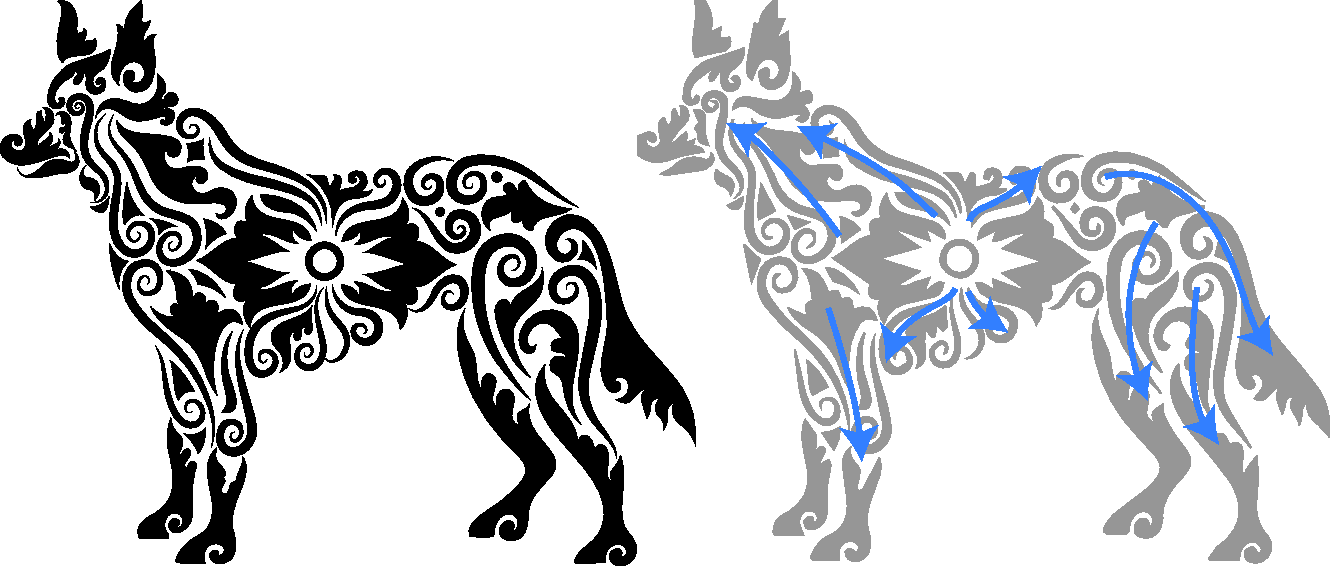
\includegraphics[width=0.6\textwidth]{figures/flowpak/dog_ornament_flow.pdf}
\vspace*{-8pt}
\caption[An example of flow visual style]{
  \label{dog_flow}  
  An example of flow visual style, 
  including a visualization of the flow directions
of elements (by ComicVector703 on Shutterstock).
}
\end{figure}

FLOWPAK~\cite{Saputra2017} is a technique for filling a container 
region with elements that are deformed 
to communicate a sense of directionality or flow.
Elements can be oriented in the local direction 
of flow, but can also be deformed to capture changes in flow direction.
Flow adds visual interest to a composition,
engaging the viewer by providing a sense of progression and
movement through elements.
A hand-drawn dog example in Fig.~\ref{dog_flow} shows many elements that appear to flow
outward from the flower in the centre of the torso, and then
up the neck and down into the legs.
Although there has been a moderate amount of past research on
the generation of packings or mosaics,
this past work is not appropriate for creating flow-like
designs similar to the dog example.

%%%%%%%%%%%%%%%%%%%%%%%%%%%%%%%%%%%%%%%%%%%%%%%%%%%%%%%%%%
%%%%%%%%%%%%%%%%%%%%%%%%%%%%%%%%%%%%%%%%%%%%%%%%%%%%%%%%%%
\section{Previous Work}
\label{flowpak_previous_work}
%%%%%%%%%%%%%%%%%%%%%%%%%%%%%%%%%%%%%%%%%%%%%%%%%%%%%%%%%%
%%%%%%%%%%%%%%%%%%%%%%%%%%%%%%%%%%%%%%%%%%%%%%%%%%%%%%%%%%




%%%%%%%%%%%%%%%%%%%%%%%%%%%%%%%%%%%%%%%%%%%%%%%%%%%%%%%%%%
%%%%%%%%%%%%%%%%%%%%%%%%%%%%%%%%%%%%%%%%%%%%%%%%%%%%%%%%%%
\section{Problem Formulation}
\label{flowpak_problem_formulation}
%%%%%%%%%%%%%%%%%%%%%%%%%%%%%%%%%%%%%%%%%%%%%%%%%%%%%%%%%%
%%%%%%%%%%%%%%%%%%%%%%%%%%%%%%%%%%%%%%%%%%%%%%%%%%%%%%%%%%

We formally define the problem to be solved as follows.  The user provides several pieces of input
to our system:
\begin{enumerate}
      \item A set of target containers.
            Each container 
			is a closed curve to be filled with ornamental elements.
      \item A set of direction guides
      		that guide the placement algorithm, defining the flow of the results. 
      		Every target container must have at least one guide, and some or
      		all of the guides typically follow the container boundaries.
      \item An optional set of fixed elements that we transfer directly to the result.
      \item A set of ornamental elements, each with a spine that will control
            its deformation.
\end{enumerate}
The first three inputs are combined into a single diagram, where they are
distinguished by their colors; see
the left and right drawings in Figure~\ref{lion_unicorn}. 
The goal of our algorithm is to fill each target container with elements,
trying to satisfy several guiding principles:
\begin{enumerate}
	\item Follow the flow defined by the direction guides.
	\item Have as little empty space as possible.
	\item Make the spacing between elements be as even as possible.
	\item Conform to container boundaries.
	\item Vary element width and length to avoid an excessively uniform arrangement.
\end{enumerate}
The next section describes how we achieve these results.

%%%%%%%%%%%%%%%%%%%%%%%%%%%%%%%%%%%%%%%%%%%%%%%%%%%%%%%%%%
%%%%%%%%%%%%%%%%%%%%%%%%%%%%%%%%%%%%%%%%%%%%%%%%%%%%%%%%%%
\section{Approach}
\label{flowpak_approach}
%%%%%%%%%%%%%%%%%%%%%%%%%%%%%%%%%%%%%%%%%%%%%%%%%%%%%%%%%%
%%%%%%%%%%%%%%%%%%%%%%%%%%%%%%%%%%%%%%%%%%%%%%%%%%%%%%%%%%


Figure~\ref{fig_flowpak_pipeline} gives an overall view of our system. The numbers in the following
steps correspond to parts of the figure.


\begin{enumerate}
  \item Read the input target containers and
  copy any fixed elements to the output art (Section~\ref{target_containers}).
  \item Analyze the ornamental elements, creating a shape descriptor for each
   (Section~\ref{ornamental_shapes}).
  \item Use the direction guides to fill each target container with a vector field then trace streamlines (Section~\ref{vector_fields_streamlines}).
  \item Divide the target containers into blobs around the streamlines (Section~\ref{subregion_blobs}).
  \item Use the element shape descriptors to determine the best element for each blob. 
        Place the element in the blob, treating it as a skeletal stroke and mapping its
        spine to the streamline (Section~\ref{shape_matching_and_deformation}).
  \item Iteratively refine the placement to eliminate empty areas and make the spacing more even (Section~\ref{iterative_refinement_process}).
\end{enumerate}

%FFFFFFFFFFFFFFF
\begin{figure}
\centering
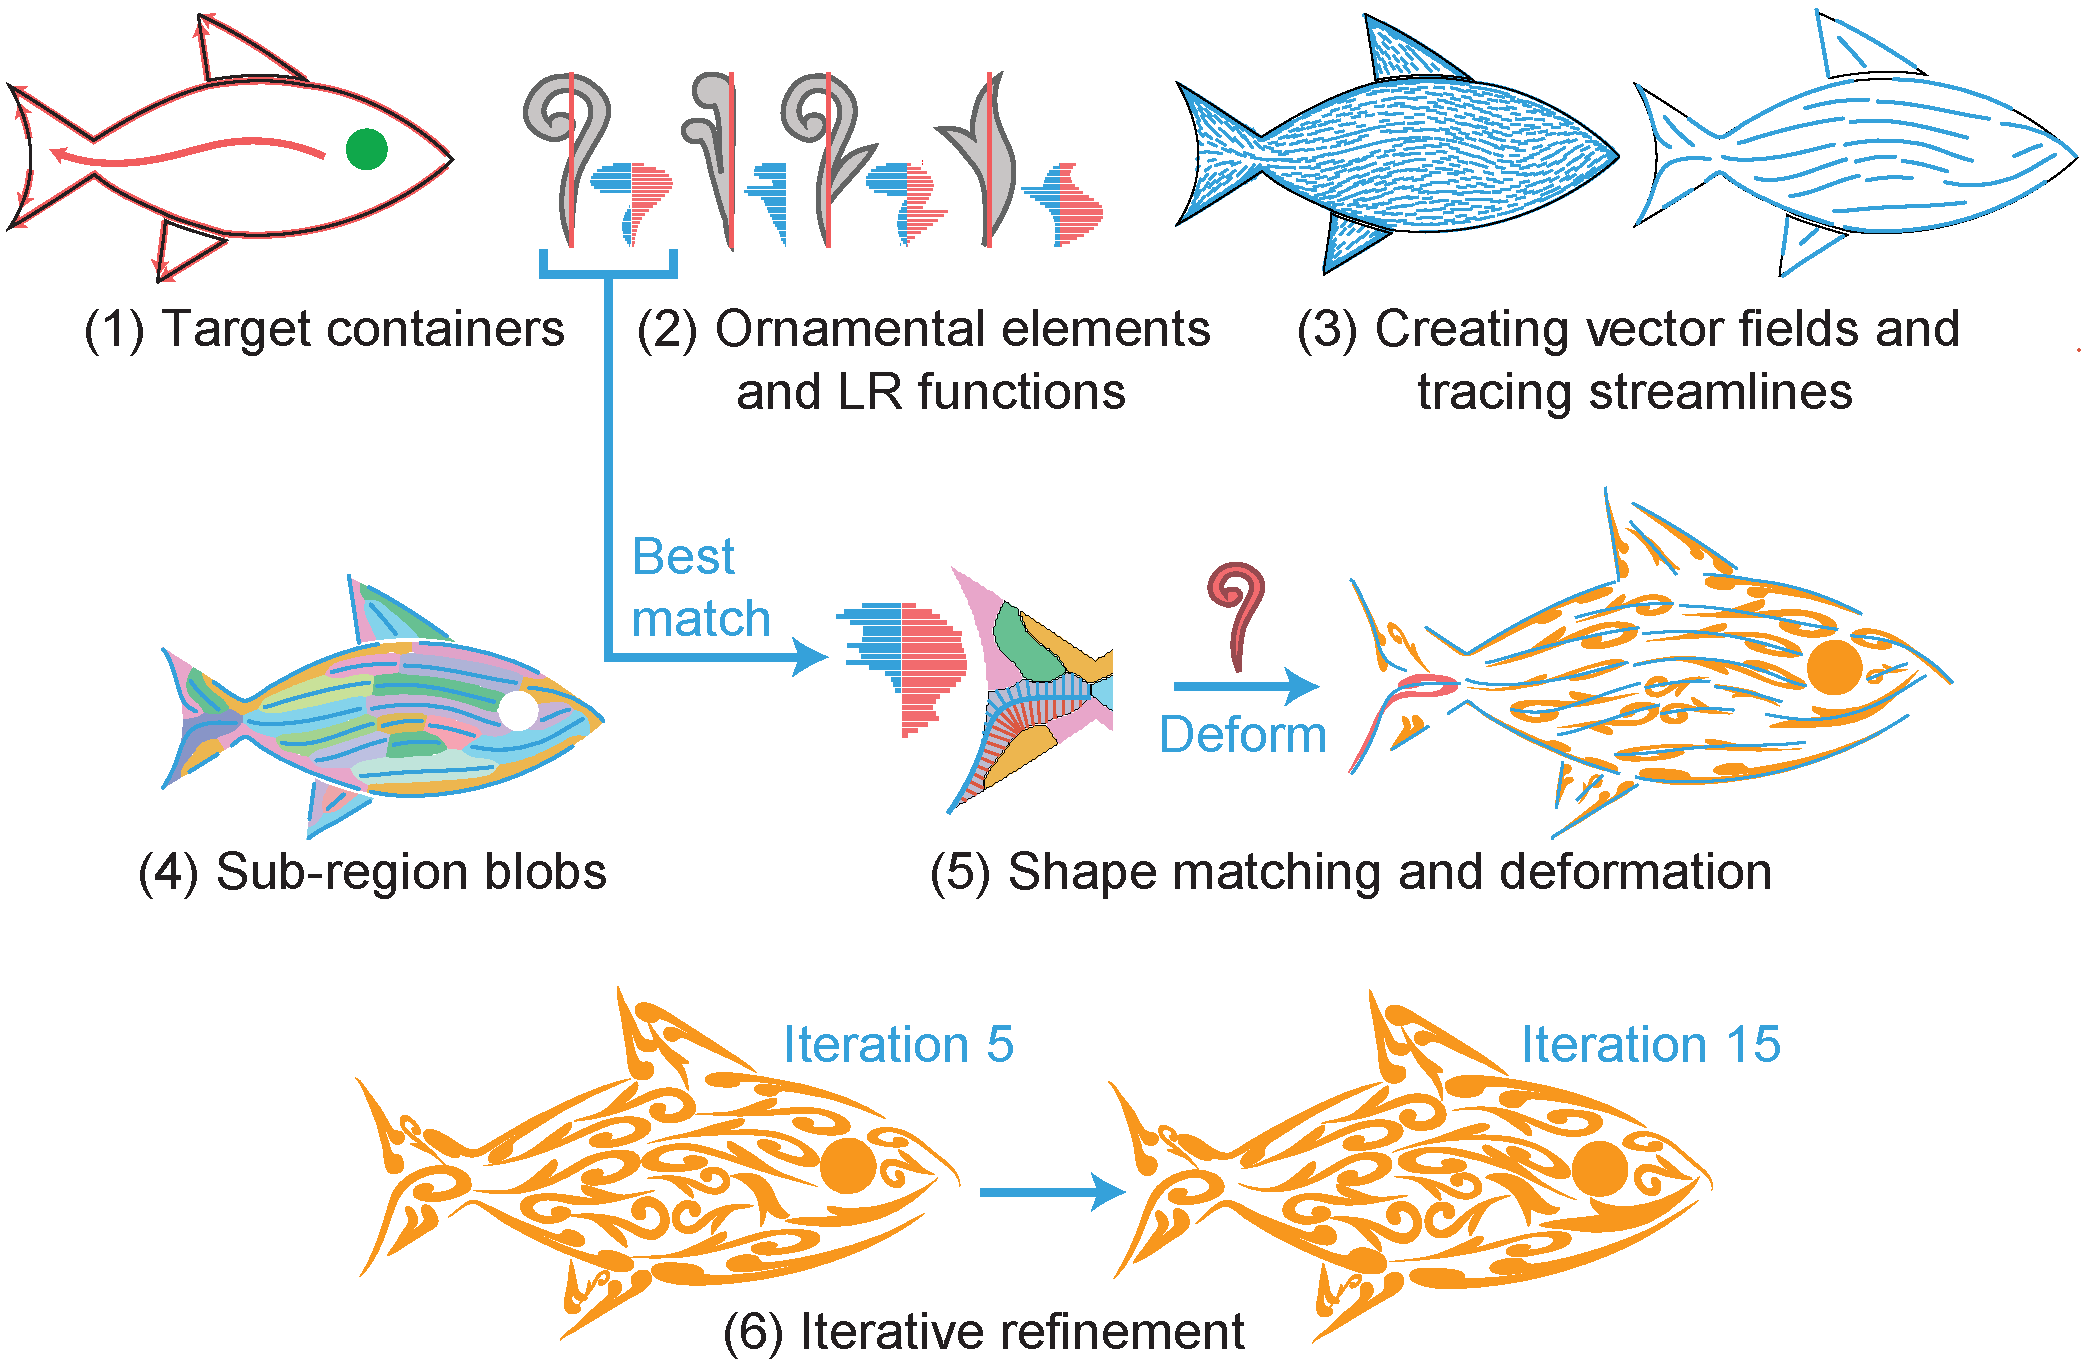
\includegraphics[width=1.0\textwidth]{figures/flowpak/pipeline.pdf} 
\caption[FLOWPAK pipeline]
{\label{fig_flowpak_pipeline} 
FLOWPAK pipeline. \mynote{Need rearrange}.}
\end{figure}

%%%%%%%%%%%%%%%%%%%%%%%%%%%%%%%%%%%%%%%%%%%%%%%%%%%%%%%%%%
%%%%%%%%%%%%%%%%%%%%%%%%%%%%%%%%%%%%%%%%%%%%%%%%%%%%%%%%%%
\subsection{Target Containers}
\label{flowpak_target_containers}
%%%%%%%%%%%%%%%%%%%%%%%%%%%%%%%%%%%%%%%%%%%%%%%%%%%%%%%%%%
%%%%%%%%%%%%%%%%%%%%%%%%%%%%%%%%%%%%%%%%%%%%%%%%%%%%%%%%%%

The input diagram contains a set of target containers. Each is a single
closed curve defining an area
to be filled.  Most non-trivial examples include more than one target
container.  For the most part, our algorithm fills each container separately,
and so the following explanation is given in terms of a single container.
Containers will later be merged in the iterative refinement step.

The artist has the option of including a set of fixed elements that
we copy directly into the final result. The following sections
include descriptions of how the fixed elements affect the filling
algorithm.

We define $input\_size$ to be the maximum of the combined width or height
of all the target containers and fixed elements as laid out by the artist.
This value will
be used to set various parameters in the synthesis process.

%%%%%%%%%%%%%%%%%%%%%%%%%%%%%%%%%%%%%%%%%%%%%%%%%%%%%%%%%%
%%%%%%%%%%%%%%%%%%%%%%%%%%%%%%%%%%%%%%%%%%%%%%%%%%%%%%%%%%
\subsection{Ornamental elements and LR functions}
\label{flowpak_ornamental_element_and_lr_functions}
%%%%%%%%%%%%%%%%%%%%%%%%%%%%%%%%%%%%%%%%%%%%%%%%%%%%%%%%%%
%%%%%%%%%%%%%%%%%%%%%%%%%%%%%%%%%%%%%%%%%%%%%%%%%%%%%%%%%%

An ornamental element is defined as one or more closed curves.  Our placement method will
eventually deform copies of the element (Section~\ref{shape_matching_and_deformation}) 
using a simple skeletal stroke algorithm~\cite{Hsu93},
so each element must be annotated with a straight spine to guide the deformation.  The spine
does not need to go through the center of the element---it can be anywhere.

We define two classes of elements: a \textit{full element} extends across
both sides of its
spine, and a \textit{half element} lies entirely on one side of its spine.
Figure~\ref{ornamental_shapes_fig} shows examples of full and half elements.  If the input
to our algorithm includes direction guides that coincide with target container boundaries,
the placement method will align half elements along these boundaries.  
If half elements 
have edges that closely follow their spines, they will visually reinforce
container boundaries, as shown in our examples.

We define a simple shape descriptor called an \textit{LR function}
that will be used in
Section~\ref{shape_matching_and_deformation} to choose which element to place in a particular location. 
Inspired by the work of Gal et al.~\cite{Gal2007A}, we sample the element's
spine at $n$ locations and at each location determine how far the ornament extends to the
left and right of the spine. The LR function is the set $\{L, R\}$ where $L=\{\ell_1,\ldots,\ell_{n\text{\_}f}\}$
is the left function and $R=\{r_1,\ldots,r_{n\text{\_}f}\}$ is the right function. The number of samples is denoted by $n\text{\_}f$.

The LR function is made scale-invariant by normalizing its
domain and range to $[0,1]$.  Note that swapping the $L$ and $R$ functions
corresponds to reflecting the element across its spine, and reversing each
of $L$ and $R$ corresponds to reflecting the element along its spine.  We
will consider all four combinations of these two reflections when placing 
an element in a blob (Section~\ref{subregion_blobs}),
in order to achieve the best possible fit.

Intuitively, LR functions give an approximate area an ornamental element can claim.
Figure~\ref{ornamental_shapes_fig} 
shows elements with their left values
in green and their right values in red. We have found that $n = 100$ gives sufficient
granularity for our algorithm.

%FFFFFFFFFFFFFFF
\begin{figure}
\centering
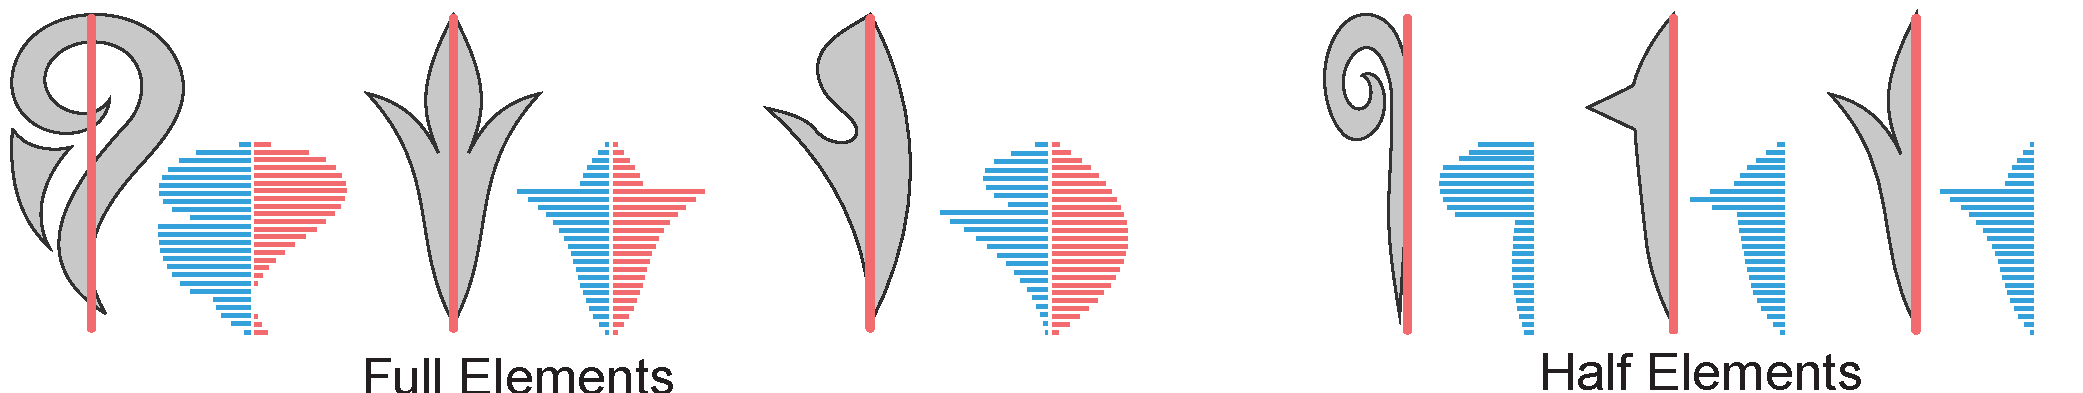
\includegraphics[width=1.0\textwidth]{figures/flowpak/ornaments.pdf}
\caption[Ornamental elements and their LR functions]
{\label{ornamental_shapes_fig}
Ornamental elements and their LR functions. Full elements have non-empty
left and right sides, while half elements have only one non-empty side. 
We normalize the LR functions to a unit square.}
\end{figure}

%%%%%%%%%%%%%%%%%%%%%%%%%%%%%%%%%%%%%%%%%%%%%%%%%%%%%%%%%%
%%%%%%%%%%%%%%%%%%%%%%%%%%%%%%%%%%%%%%%%%%%%%%%%%%%%%%%%%%
\subsection{Creating Vector Fields and Tracing Streamlines}
\label{flowpak_creating_vector_fields_and_tracing_streamlines}
%%%%%%%%%%%%%%%%%%%%%%%%%%%%%%%%%%%%%%%%%%%%%%%%%%%%%%%%%%
%%%%%%%%%%%%%%%%%%%%%%%%%%%%%%%%%%%%%%%%%%%%%%%%%%%%%%%%%%

To implement the flow principle described in the introduction, we fill each target
container with a vector field, constrained by the direction guides in that container.

We sample the directional guides $D = \{ d_{1}, d_{2}, ... , d_{n\text{\_}d}\}$  
and use the tangent at every sampled point as a directional constraint.
We then construct a vector field using the $N$-RoSy algorithm
of Palacios and Zhang\cite{Palacios2007}.  Note that, as shown in 
Step~3 of Figure~\ref{pipeline},
fixed elements do not affect the vector field.  
The artist can include directional guides to guide the vector field around fixed elements if desired.

The next step is to trace streamlines in the vector field, guided by three input parameters:
\begin{conditions}
d\_gap \enspace & the desired space between streamlines \\
s\_max & the maximum desired streamline length \\
s\_min & the minimum desired streamline length   
\end{conditions}
Because we will ultimately place elements along streamlines without overlap, $d\_gap$ determines
the approximate width of the placed elements, and $s\_max$ the maximum length.  We also derive
a value $d\_stop$ that prevents streamlines from coming too close to each other; in our implementation we
compute $d\_stop = 0.8\,d\_gap$.

We adapt the streamline tracing algorithm of Jobard and Lefer~\cite{Jobard1997}.
First we generate a set of potential seed points $P = \{ p_{1}, p_{2}, ... , p_{n\text{\_}p}\}$  by
densely resampling the target container boundary $T$ and the directional guides in $D$.
We use a sampling distance of $0.005\,input\_size$.
The first streamline $s$ is generated by randomly removing a seed point from $P$ and following
the vector field until one of the following conditions holds:

\begin{enumerate}
\item the length of $s$ would exceed $s\_max$.
\item $s$ would come within $d\_stop$ of another streamline.
\item $s$ would cross $T$, leaving the container.
\item $s$ would cross the boundary of a fixed element.
\end{enumerate}


If the length of $s$ is less than $s\_min$, we discard it. Otherwise we sample 
$s$, again using $0.005\,input\_size$, and at each point generate two more
potential seeds that are $d\_gap$ away from $s$ on either side. If a seed is
inside the container, we add it to $P$.  The process is repeated until $P$ is empty.
Note that the $d\_stop$ distance test combined with the $s\_min$ length
test imply that many attempts to form streamlines will stop immediately,
especially as the container fills with streamlines.

Figure~\ref{streamline_tracing} shows the creation process, and 
Algorithm~\ref{tracing_streamlines} shows the pseudocode.
The sort function \textsc{Sort}$(P)$ orders the points in $P$ according to their distance from the
boundary $T$ and the directional guides in $D$, with closer points first and equally distant
points ordered randomly. Because the initial points are all on $T$ or on a path in $D$, their
sort value is zero, and they will be processed before any derived points. 

\begin{algorithm}[h!]
\caption{Tracing streamlines} 
\label{tracing_streamlines}
\begin{algorithmic} 
\STATE Create a seed list $P = \{ p_{1}, p_{2}, ... , p_{n\text{\_}p}\}$ 
       by uniformly resampling
\STATE \hskip\algorithmicindent $T$ and the guides in $D$.
\STATE Create an empty set $S$ of streamlines.
\STATE Randomly order the elements of $P$.
\WHILE {$P$ is not empty}
  \STATE Generate a new streamline $s$ from $p_{1}$.
  \STATE Remove $p_{1}$ from $P$.
  \IF {$s$ is longer than $s\_min$}
    \STATE Add $s$ to $S$.
    \STATE Create seed points that are $d\_gap$ away from $s$ and
	\STATE \hskip\algorithmicindent add them to $P$.
    \STATE \textsc{Sort}$(P)$.
  \ENDIF
\ENDWHILE
\end{algorithmic}
\end{algorithm}

%FFFFFFFFFFFFFFF
\begin{figure}
\centering
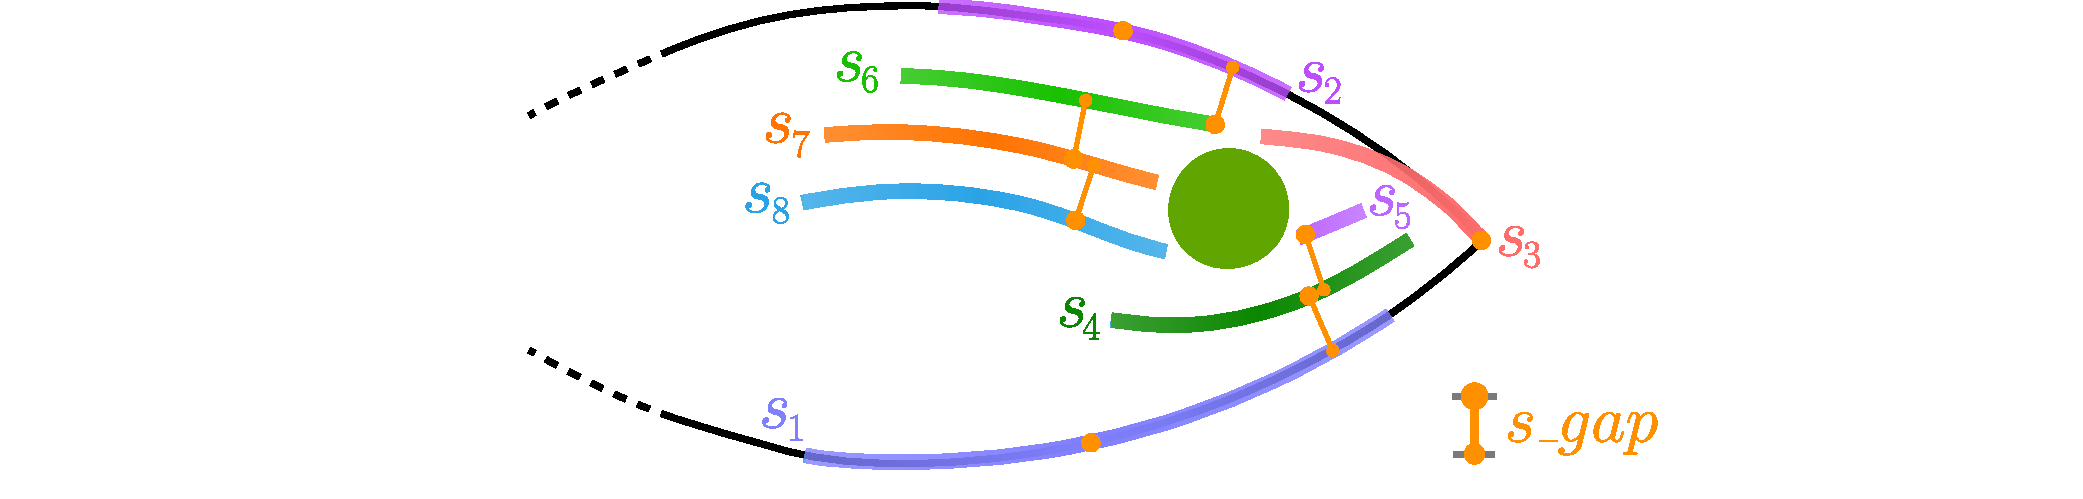
\includegraphics[width=1.0\textwidth]{figures/flowpak/streamline_tracing.pdf}
\caption[The streamline tracing process]
{\label{streamline_tracing}
The streamline tracing process. The first streamline $s_1$ always begins
on a directional guide or the container boundary.  Subsequent streamlines begin
on the container boundary, a directional guide, or at a point that is 
$d\_gap$ away from a previous streamline.}
\end{figure}

%%%%%%%%%%%%%%%%%%%%%%%%%%%%%%%%%%%%%%%%%%%%%%%%%%%%%%%%%%
%%%%%%%%%%%%%%%%%%%%%%%%%%%%%%%%%%%%%%%%%%%%%%%%%%%%%%%%%%
\subsection{Sub-region blobs}
\label{flowpak_sub-region_blobs}
%%%%%%%%%%%%%%%%%%%%%%%%%%%%%%%%%%%%%%%%%%%%%%%%%%%%%%%%%%
%%%%%%%%%%%%%%%%%%%%%%%%%%%%%%%%%%%%%%%%%%%%%%%%%%%%%%%%%%

To assist in choosing which element to place along each streamline, we first
subtract the areas of any fixed elements from the target container. We then
construct an approximate generalized Voronoi diagram of the interior
using the method of Osher and Sethian~\cite{Osher1988}.
The streamlines are then extended at each end, following the vector field, until
they encounter the boundaries of their Voronoi regions.
We call the area around each streamline a \textit{sub-region blob}.
Step~4 of Figure~\ref{pipeline} 
shows the blobs for the sample fish.

We then compute an LR function for each blob as described in Section~\ref{ornamental_shapes},
using the streamline as the spine. Because the streamline is not usually straight, we 
compute the left and right distances along the normals to the streamline. The LR function approximates
the blob's shape if the streamline were to be straightened.

%%%%%%%%%%%%%%%%%%%%%%%%%%%%%%%%%%%%%%%%%%%%%%%%%%%%%%%%%%
%%%%%%%%%%%%%%%%%%%%%%%%%%%%%%%%%%%%%%%%%%%%%%%%%%%%%%%%%%
\subsection{Shape Matching and Deformation}
\label{flowpak_shape_matching_and_deformation}
%%%%%%%%%%%%%%%%%%%%%%%%%%%%%%%%%%%%%%%%%%%%%%%%%%%%%%%%%%
%%%%%%%%%%%%%%%%%%%%%%%%%%%%%%%%%%%%%%%%%%%%%%%%%%%%%%%%%%

The next step is to place an ornamental element in each blob.  We choose which element
to place in the blob by finding the element that minimizes a sum of least squares distance, defined as
%\vspace{-4pt}
\begin{equation}
\sum_{i=1}^{N} (\alpha_{li} - \beta_{li})^2 + \sum_{i=1}^{N} (\alpha_{ri} - \beta_{ri})^2
\end{equation}
where
%\vspace*{-4pt}
\begin{conditions}
\alpha_{l}\enspace & the element left function\\
\alpha_{r} &  the element right function \\   
\beta_{l}  &  the blob left function \\
\beta_{r}  &  the blob right function
\end{conditions}
%\vspace{-4pt}

Every element can be placed in one of four orientations, by optionally 
incorporating reflections across and along its spine.  These reflections
correspond, respectively, to swapping the $L$ and $R$ functions and reversing
them.  When comparing the LR functions for an element and a blob, we compute
the least squares distances for all four orientations and choose the 
orientation with the smallest distance.  Note that this matching method
automatically places half elements along streamlines that follow container
boundaries, visually reinforcing the overall shape.

We investigated alternatives for shape matching, using an approach
discussed by Gal et al. \cite{Gal2007B} that tries to fill a sub-region
blob as much as possible, with heavy penalties if a part of an
element protrudes outside the boundary of the blob. However, we found
this computation to be more expensive without providing significant
advantages over our LR functions.

Once we have chosen an element, we place it along the streamline using a
simple skeletal stroke algorithm~\cite{Hsu93}. We uniformly scale the element's width
to make it as wide as possible while still staying inside the blob
(Figure~\ref{shape_deformation}).

%FFFFFFFFFFFFFFF
\begin{figure}
\centering

\includegraphics[width=6.4cm]{figures/flowpak/shape_deformation.pdf}
\caption[Shape deformation]
{\label{shape_deformation}
The deformation process bends the element along the streamline and
scales it to fit inside the blob.}
\bigskip
 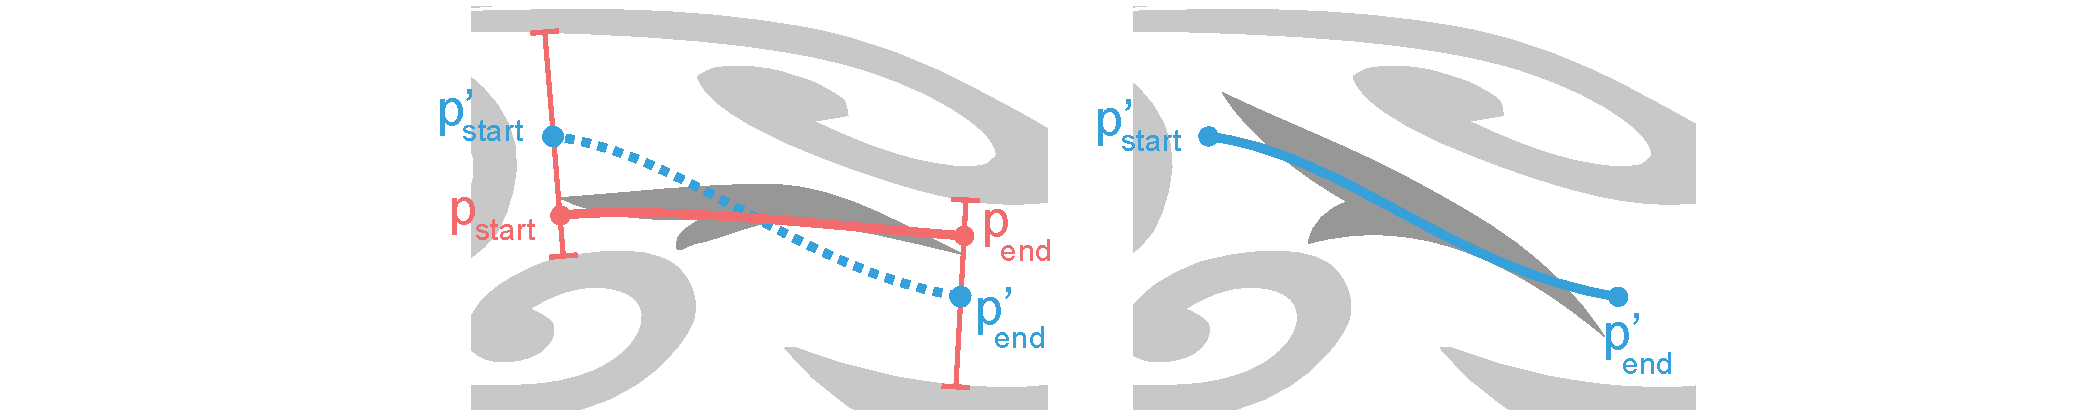
\includegraphics[width=6.4cm]{figures/flowpak/shift_streamline.pdf}
 \caption[Shift a streamline]
 {\label{shift_streamline}
 Streamline shifting.
 	We move the streamline's start and end points along 
	perpendiculars, stopping before intersecting neighbouring elements.}
\smallskip

\includegraphics[width=3.2cm]{figures/flowpak/dijkstra.pdf}
 \caption[Trace a shortest path]
 {\label{dijkstra}
 Tracing a shortest path using Dijkstra's algorithm.  We generate the 
 orange nodes by resampling and offsetting the original red streamline.
          The search directions at a node are shown with green arrows.}
\end{figure}

Once we have chosen an element, we place it along the streamline using a
simple skeletal stroke algorithm~\cite{Hsu93}. We uniformly scale the element's width
to make it as wide as possible while still staying inside the blob
(Figure~\ref{shape_deformation}).

%%%%%%%%%%%%%%%%%%%%%%%%%%%%%%%%%%%%%%%%%%%%%%%%%%%%%%%%%%
%%%%%%%%%%%%%%%%%%%%%%%%%%%%%%%%%%%%%%%%%%%%%%%%%%%%%%%%%%
\subsection{Iterative Refinement}
\label{flowpak_iterative_refinement}
%%%%%%%%%%%%%%%%%%%%%%%%%%%%%%%%%%%%%%%%%%%%%%%%%%%%%%%%%%
%%%%%%%%%%%%%%%%%%%%%%%%%%%%%%%%%%%%%%%%%%%%%%%%%%%%%%%%%%

We now refine the overall composition in an iterative process.  We perform
this part of the algorithm globally, by merging all containers and allowing the
elements within them to interact.

The refinement process aims to reduce the amount of negative space and make it
more even by growing and shifting the placed ornamental elements. It would be 
possible to use a greedy approach, improving the placement of each element as much
as possible before moving on to the next, However, we have found that gradually
improving the placement of all elements leads to a more even result.

Each refinement
iteration has two phases.
First, we shift the streamlines to more accurately follow the space that is available,
as shown in Figure~\ref{shift_streamline}. After shifting, we recalculate the LR function
for the blob to reflect the new position, and repeat a variant of the
element placement process
that allows the elements to rotate slightly in their space.
Second, we expand each blob to allow it to use adjacent space that is not 
filled with another element, as shown in Figure~\ref{stretch_ornament}.

Each refinement iteration considers the blobs in increasing order of 
placed element area, allowing smaller elements to grow more.   While each step
usually results in a larger placed element, some
configurations can result in a smaller one. We only accept the new element if its
area is no smaller than $\alpha$ times its old area, where $\alpha$ is a growth tolerance
that we set to $0.9$. Elements therefore have some freedom to grow or
shrink, in the search for more globally even spacing.

Algorithm~\ref{iterative_refinement_algorithm}
gives the overall method, and the following sections give details. We have found that
15 iterations suffice for most designs.
Note that in Algorithm~\ref{iterative_refinement_algorithm}, the variable
$E$ is the list of placed, distorted ornamental elements, and
not the set of prototype elements discussed earlier.

\begin{algorithm}[t] 
\caption{Iterative refinement} 
\label{iterative_refinement_algorithm}
\begin{algorithmic} 
\REQUIRE $E = \{ e_{1}, e_{2},... , e_{n\text{\_}e} \}$ as the ornamental element list. 
\REQUIRE $S = \{ s_{1}, s_{2},... , s_{n\text{\_}s} \}$ as the streamline list.
\REQUIRE $B = \{ b_{1}, b_{2},... , b_{n\text{\_}b} \}$ as the blob list.
\REQUIRE $\alpha$ as the growth tolerance
\REQUIRE $t$ as the number of iterations
\FOR {$t$ times}

  \STATE Sort $E$, $S$, and $B$ by \textsc{Area}$(e_{i})$ (smallest first)
  \FOR {Element $e_{i}$ in $E$}
  	\STATE $s_{i}$ is the corresponding streamline of $e_{i}$
    \STATE Calculate $s'_{i}$ by \textbf{shifting} $s_{i}$.
    \STATE Recompute the LR function of $b_{i}$ to give $b'_{i}$
    \STATE Calculate $e'_{i}$ by \textbf{placing} $e_{i}$ inside $b'_{i}$
    \IF{$\textsc{Area}(e'_{i}) \times \alpha > \textsc{Area}(e_{i})$}
        \STATE $s_{i} \leftarrow s'_{i}$
        \STATE $b_{i} \leftarrow b'_{i}$
    	\STATE $e_{i} \leftarrow e'_{i}$ 
    \ENDIF
  \ENDFOR
  \STATE Sort $E$, $S$, and $B$ by \textsc{Area}$(e_{i})$ (smallest first)

  \FOR {Element $e_{i}$ in $E$}
  	\STATE $b_{i}$ is the corresponding blob of $e_{i}$
    \STATE Calculate $b'_{i}$ by \textbf{growing} $b_{i}$.
    \STATE Calculate $s'_{i}$ based on $b'_{i}$ 
    \STATE Calculate $e'_{i}$ by \textbf{placing} $e_{i}$ inside $b'_{i}$\
    \STATE $b_{i} \leftarrow b'_{i}$
    \IF{$\textsc{Area}(e'_{i}) \times \alpha > \textsc{Area}(e_{i})$}
        \STATE $s_{i} \leftarrow s'_{i}$
    	\STATE $e_{i} \leftarrow e'_{i}$ 
    \ENDIF
  \ENDFOR

\ENDFOR
\end{algorithmic}
\end{algorithm}

\textbf{Shifting streamlines.}
There are two issues that keep the initial placement of elements from being
evenly
distributed. Our streamline placement method keeps streamlines apart,
but they may not be spaced completely evenly. More significantly, the
ornamental elements often have unbalanced left and right sides and concavities,
leading to extra space on one side or the other.  Our refinement process
shifts streamlines to address these problems.

The shifting process allows the endpoints of the streamline to move to the
left or the right relative to the streamline, depending on which side has more empty space.
This allows the streamline's element to become wider and fill more of the space
(Figure~\ref{shift_streamline}). It also gives the streamline room to
extend if its endpoints were too close to boundaries of other placed
elements.

Given the endpoints $p_\mathrm{start}$ and $p_\mathrm{end}$, we 
calculate new endpoints $p'_\mathrm{start}$ and $p'_\mathrm{end}$.
We generate perpendicular
vectors to the left side and to the right side at each endpoint and construct
a line segment joining the points where the vectors intersect other placed elements.
We then move the endpoint of the streamline towards the midpoint of this
segment. To enforce the principle of gradual refinement, we do not allow the
endpoint to move more than $g_\mathrm{limit}$ units, where 
$g_\mathrm{limit}=0.005\,input\_size$ (Recall that $input\_size$ is the maximum dimension
of the design as described in Section~\ref{target_containers}).

We replace the streamline with a path joining
$p'_\mathrm{start}$ and $p'_\mathrm{end}$. Our goal
is to create a path that is smooth and does not deviate too much from the vector
field.  We calculate the shifted streamline by performing Dijkstra's
algorithm on a non-rectangular graph that respects the vector field
(Figure~\ref{dijkstra}), using a method similar to one by Xu and Mould~\cite{Mould2015} for
pathfinding in a vector field.

To construct the graph, we begin by densely sampling the original
streamline with a distance of $0.25\,g_\mathrm{limit}$. We then duplicate
the points, offset to the left and right, again using $0.25\,g_\mathrm{limit}$.
The duplication is repeated until the graph extends to the left and right of the
streamline by a distance equal to the maximum left and right widths of the blob (i.e.,
the maximum values in an unnormalized version of the blob's LR function).

For a node, we check its $N = 150$ nearest neighbors, considering only neighbors where the angle between the line into the current node and the line to the neighbor form an angle greater than $90^\circ$, thereby preventing
the streamline from backtracking.
The cost of an edge from $n_a$ to  $n_b$ is 

\begin{equation}
w = w_f (1 - f^p) + w_d \: D(s_i, n_a)
\end{equation}
where
\begin{conditions}
f                  & $(n_b-n_a) \cdot \vec{v}$ \\
\vec{v} 		   & a sampled vector of the vector field \\
s_i                & the original streamline \\   
D()\enspace        & a distance function between a polyline and a point
\end{conditions}

In practice, we set $w_d = 0.1$, $w_f=1$, and $p = 3$.

After finding a set of points, we fit cubic B\'ezier curves using a method
devised by Schneider \cite{Schneider1990} and extend the path at both ends 
by following
the vector field until it intersects the edges of its blob. 

\textbf{Growing blobs.} The growth process tries to enlarge each sub-region blob to
claim empty space.
Given a blob $b_{i}$, we calculate a larger blog $b'_{i}$ 
by offsetting its boundaries until they intersect other placed elements (Figure~\ref{stretch_ornament}).
To enforce gradual growth, the offset cannot be larger than $g_\mathrm{limit}$, where
$g_\mathrm{limit}=0.005\,input\_size$.

The value $g_\mathrm{limit}$ used in growing blobs and shifting streamlines limits the speed of
the refinement.  Making it larger would require fewer iterations to fill the available space,
but at a cost of elements growing less evenly. 

% ROTATING OR FLIPPING
\textbf{Element placement.}
In the refinement process, we allow a more flexible element placement so that
the elements can fill more of their blobs.  We allow the element
to rotate by a small amount, up to ten degrees, before placing it, as shown in
Figure~\ref{rotate_ornament}. 
We generate rotated versions of $e_{i}$ 
with varying angles $r_\mathrm{angle} = {1^{\circ}, 2^{\circ}, 3^{\circ}, ..., 10^{\circ}}$
and precompute LR functions for each. The shape matching algorithm
(Section~\ref{shape_matching_and_deformation}) automatically choses the best rotation. It
can also choose to reflect the element across its spine, along its spine, or both (Figure~\ref{flip_shape})

%FFFFFFFFFFFFFFF
\begin{figure}[t]
\centering

\includegraphics[width=6.5cm]{figures/flowpak/stretch.pdf}
\caption[Enlarge an element]
{\label{stretch_ornament}
(a) An element with its sub-region blob shown in dashed green line. Note that any blob is constrained by the neighboring elements. 
(b) The dashed red line is the grown blob, which accommodates an enlarged element.}

% ROTATING OR FLIPPING
\medskip
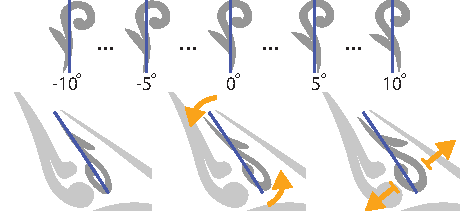
\includegraphics[width=6.5cm]{figures/flowpak/rotate_ornament.pdf}
\caption[Rotate an element]
{\label{rotate_ornament}
Top row: rotated versions of the original element. 
         The best rotation angle is chosen via least squares matching.
         Bottom row: original, rotated, and enlarged versions of an element.}

\medskip
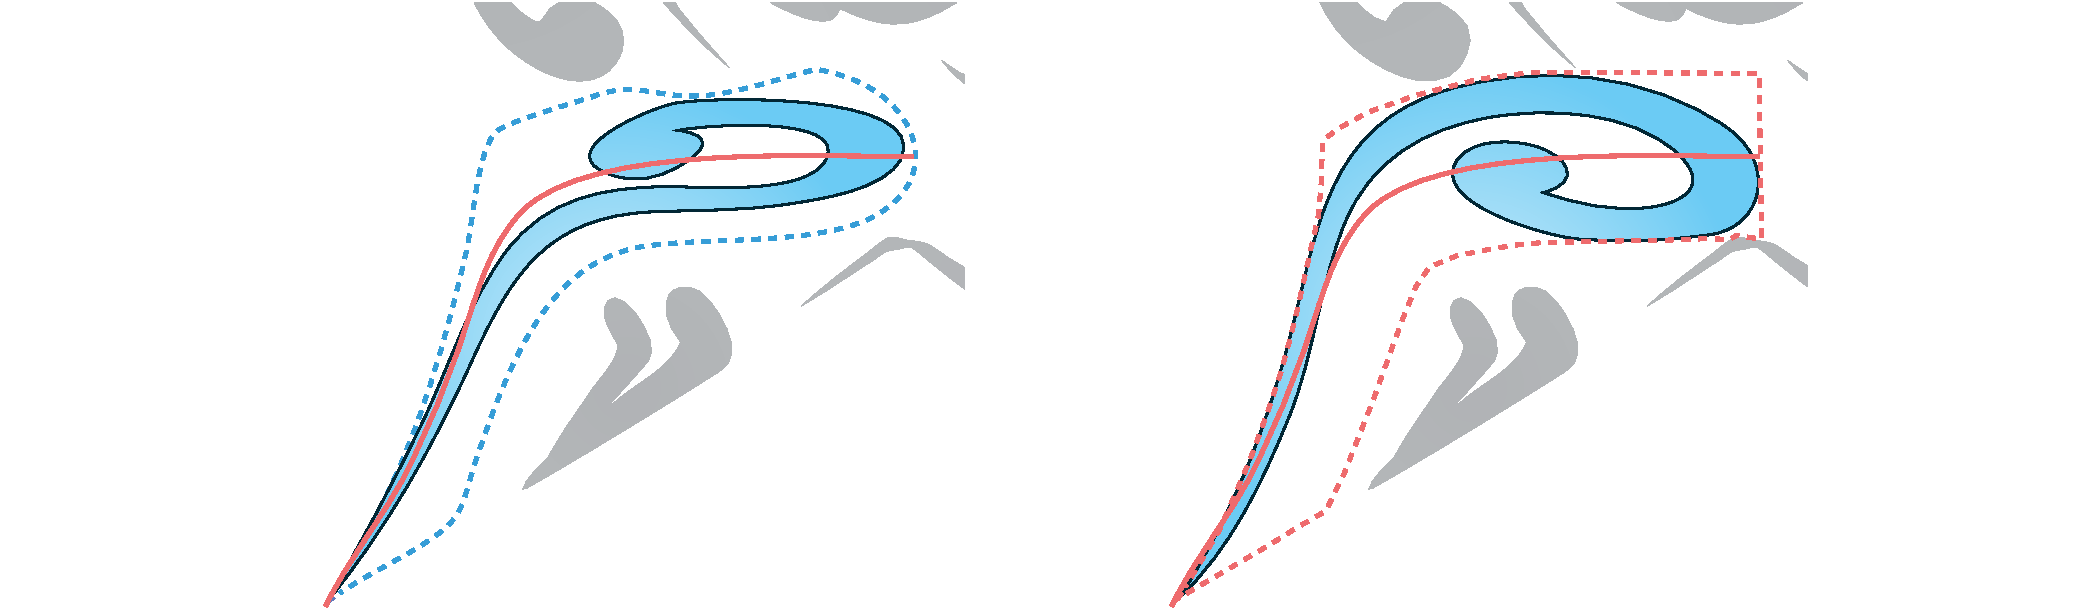
\includegraphics[width=4.5cm]{figures/flowpak/flip.pdf}
\caption[Flip an element]
{\label{flip_shape}
An element that reflects across its spine during iterative refinement.
LR functions and least squares shape matching allow an element to reflect
across its spine, along its spine, or both.}
\end{figure}

%%%%%%%%%%%%%%%%%%%%%%%%%%%%%%%%%%%%%%%%%%%%%%%%%%%%%%%%%%
%%%%%%%%%%%%%%%%%%%%%%%%%%%%%%%%%%%%%%%%%%%%%%%%%%%%%%%%%%
\section{Implementation and Results}
\label{flowpak_implementation_and_results}
%%%%%%%%%%%%%%%%%%%%%%%%%%%%%%%%%%%%%%%%%%%%%%%%%%%%%%%%%%
%%%%%%%%%%%%%%%%%%%%%%%%%%%%%%%%%%%%%%%%%%%%%%%%%%%%%%%%%%

We design our containers and decorative elements in a vector graphics 
editor, and then use them as input to a C++ program that outputs final
placed elements in an SVG file.  We use the Clipper library~\cite{ClipperLib}
for calculation of LR functions and for testing polygon intersections 
during deformation and growth.
As a postprocess, we optionally smooth outlines and replace polygonal
paths with B\'{e}zier curves.
Finally, we apply colours and other treatments in an editor.

Our technique is fast except for the iterative refinement process,
which considers a large number of variations to the composition via
brute-force computation. On a computer with an Intel i7-4790K processor at 4.0 Ghz,
 15 iterations
of refinement on a packing of 50 elements takes about an hour.  Our
software is not intended to run interactively; still, we believe the
performance could be improved significantly through the use of more
sophisticated 2D geometric data structures like quadtrees.

We tested our approach using a variety of container shapes, based mostly
on animals, and many different ornamental elements with varying amounts
of geometric complexity.
In Figure~\ref{result_rhino},
we show a packing of a rhinoceros with simple teardrop elements
that demonstrates the variety we achieve in shape and curvature.
We use more complex leaf elements on the bear in 
Figure~\ref{result_bear_leaves}, and
adjust the tracing parameters to obtain shorter placed elements. 
We also process the placed elements to create a distressed look.


The packing of a cat in Figure~\ref{result_cat} demonstrates a symmetric packing with
a fur contour inspired by Figure~\ref{some_examples}c. 
We only compute the left part and reflect the result.
The elements around the cheeks and the chin extend outward, not following the boundary, and creating the appearance of fur.

We experimented with two extensions to our pipeline, 
which could enhance its aesthetic value and flexibility.
First, in Figure~\ref{result_dog} we allow the user to draw 
\textit{fixed spines} in addition to fixed elements.  These fixed
spines act like pre-placed streamlines, which will be assigned blobs
and then elements.  However, they are not required to follow the
surrounding vector field, and are not shifted during the refinement
process.  Fixed spines are used in Figure~\ref{result_dog} for the 
flower petals in the torso and the paws.
Second, in Figure~\ref{result_bear_offset} we construct explicit new shapes
(drawn in brown)
to fill the negative space between placed elements (in black), 
by computing offset polygons from the negative space between elements. 
The result is a distinct and appealing style.  

Finally, we asked an artist to draw containers and a decorative elements.
The result is the bird design shown in Figure~\ref{bird_square}.
The artist requested that different elements and densities be used in 
different container regions; the result has sparse ``Y'' elements in 
the breast and head, and denser ``O'' elements in the wings. The artist was pleased with the results.

%FFFFFFFFFFFFFFF
\begin{figure}
\centering
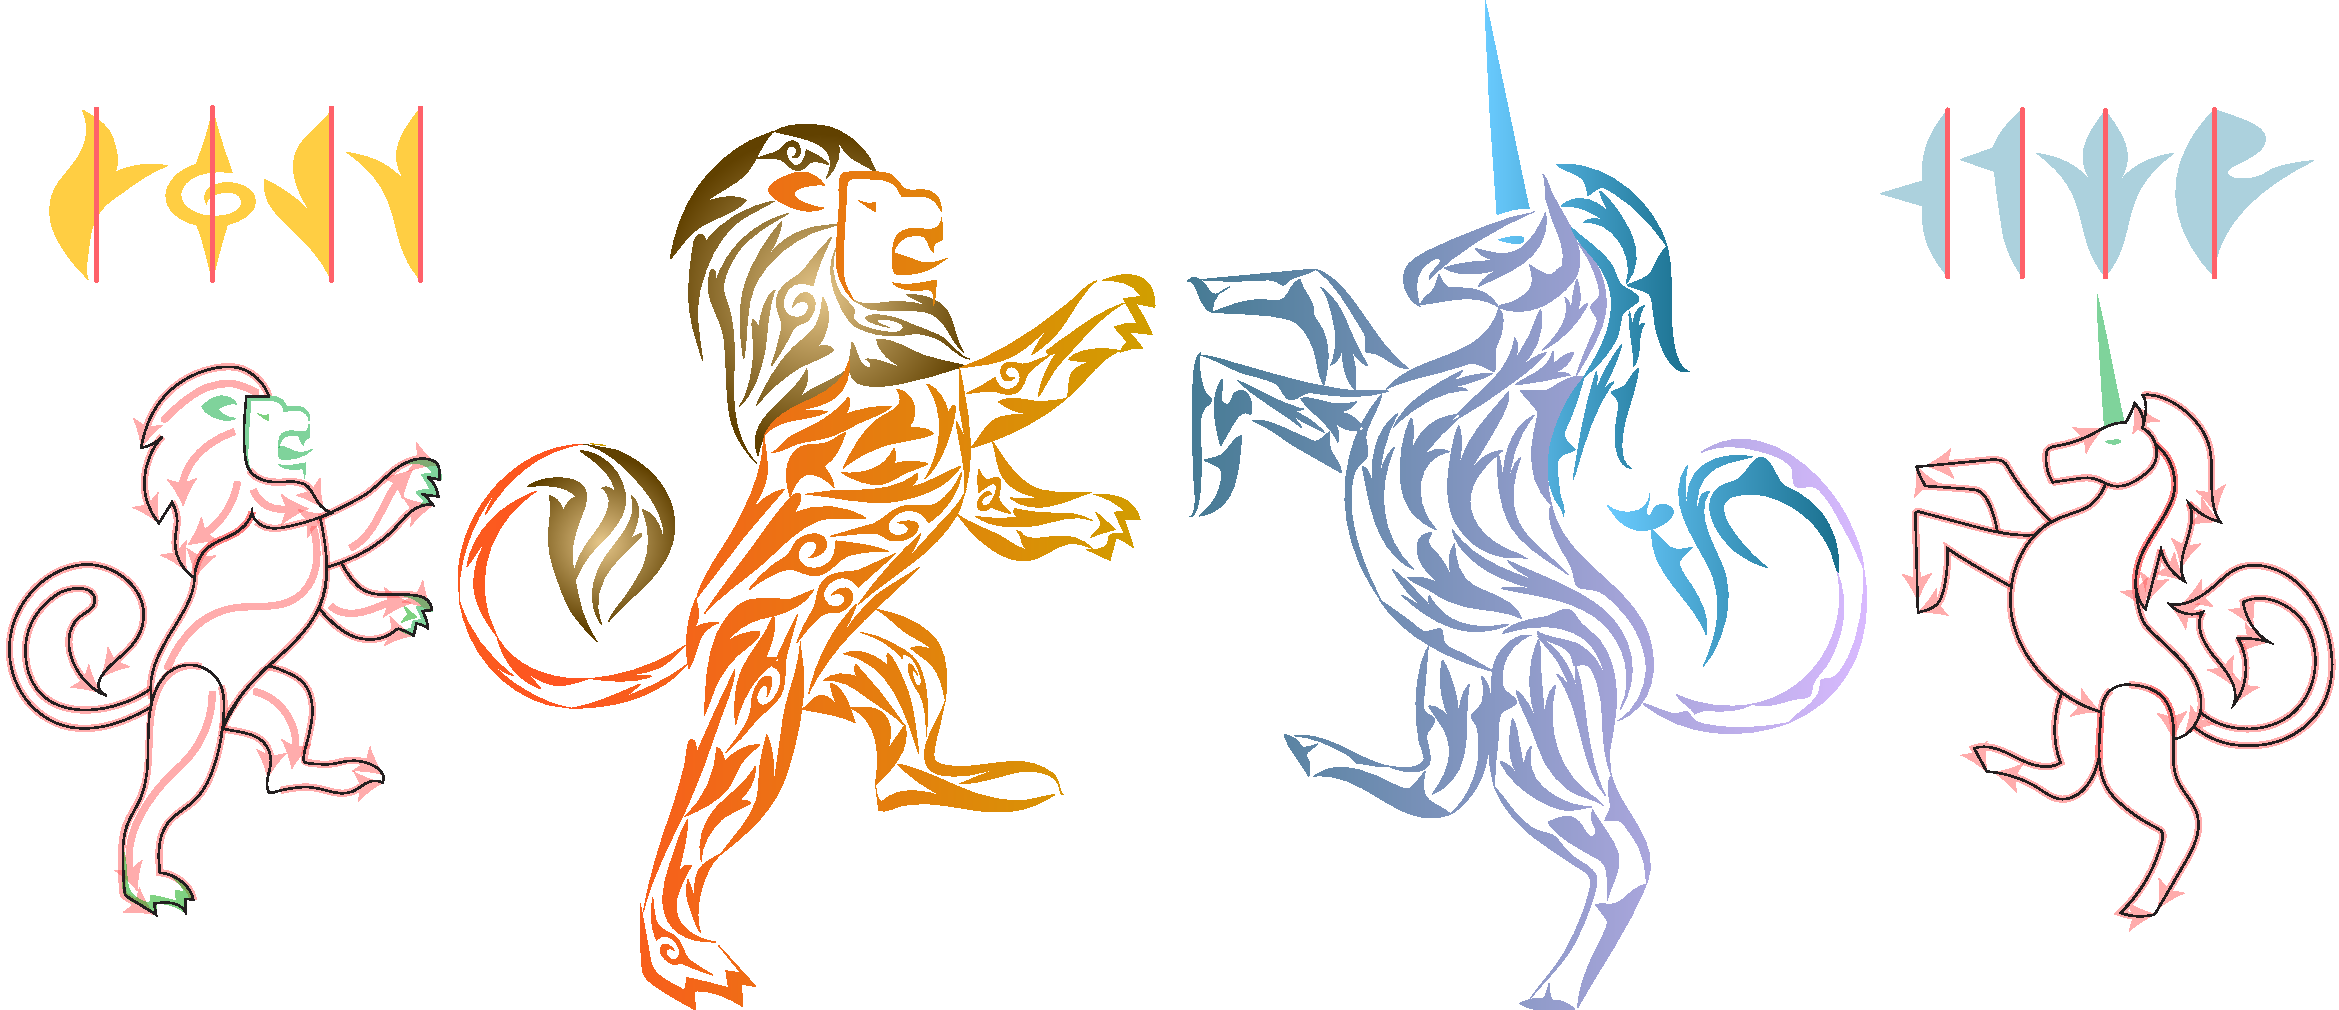
\includegraphics[width=1.0\textwidth]{figures/flowpak/lion_unicorn.pdf} 
\caption[A packing of lion and unicorn]
{\label{fig_lion_unicorn} 
Lion Unicorn. }
\end{figure}

%FFFFFFFFFFFFFFF
\begin{figure}[t!]
\centering
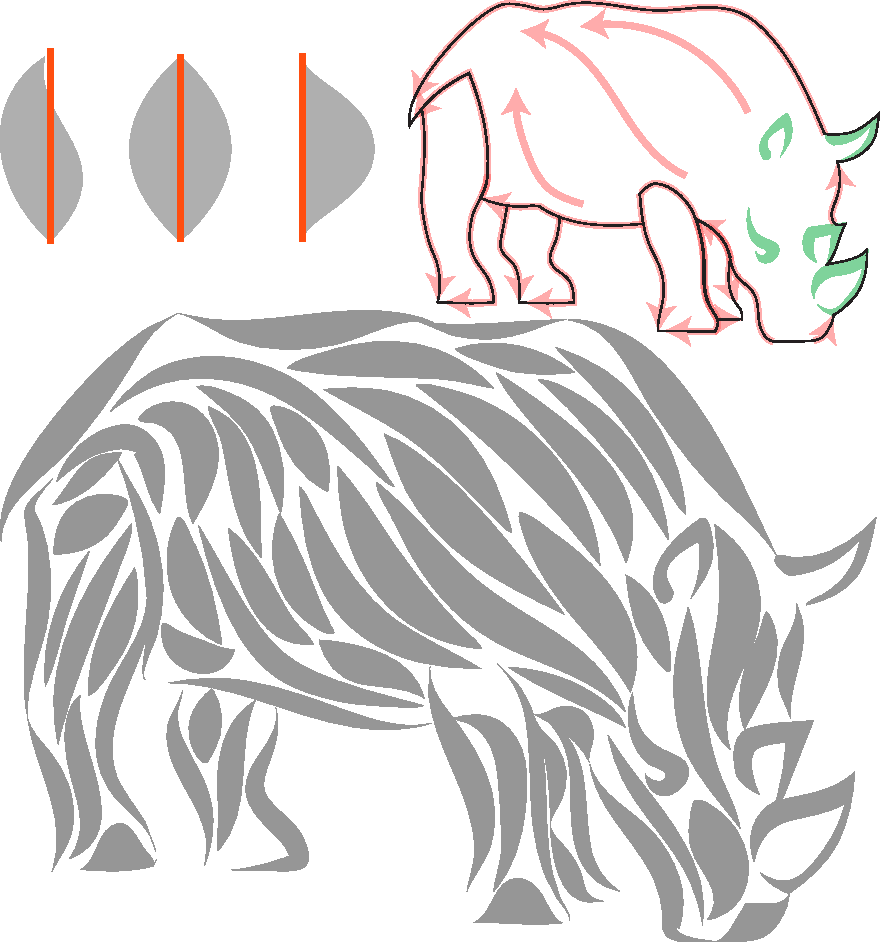
\includegraphics[width=5cm]{figures/flowpak/result_02.pdf} %RHINO
\caption[A packing of a rhinoceros]
{\label{result_rhino}
A packing of a rhinoceros.  Simple teardrop-shaped 
elements lead to variety in size and curvature.}
\bigskip
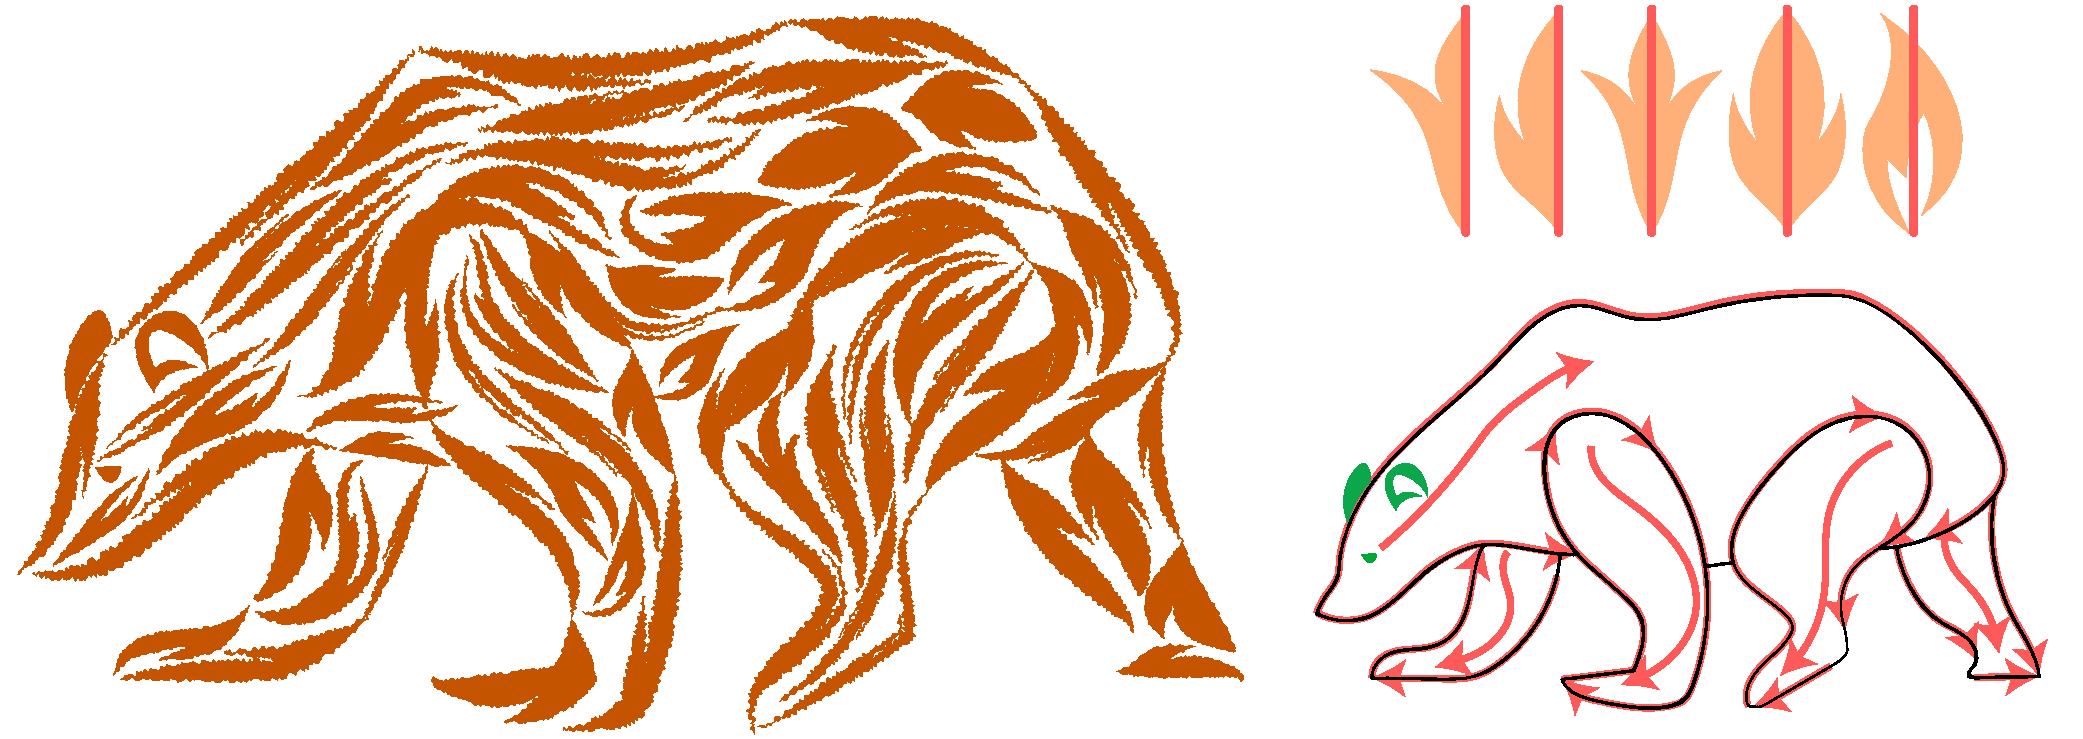
\includegraphics[width=6cm]{figures/flowpak/bear_leaves.pdf} %BEAR LEAVES
\caption[A packing of a bear with leaf elements]
{\label{result_bear_leaves}
	A bear packing with leaf elements.  We manually add noise to the 
	elements in the output to create a distressed look.}
\end{figure}

%FFFFFFFFFFFFFFF
\begin{figure} %CAT
\centering

\includegraphics[width=6.5cm]{figures/flowpak/cat.pdf}
\caption[A packing of a cat]
{A packing with a symmetric layout; we only compute the left half and reflect the result. The elements around the cheeks and the chin are not aligned to the boundary, creating a fur-like effect.}
\label{result_cat}
\end{figure}

%FFFFFFFFFFFFFFF
\begin{figure} %DOG FLOWER
\centering
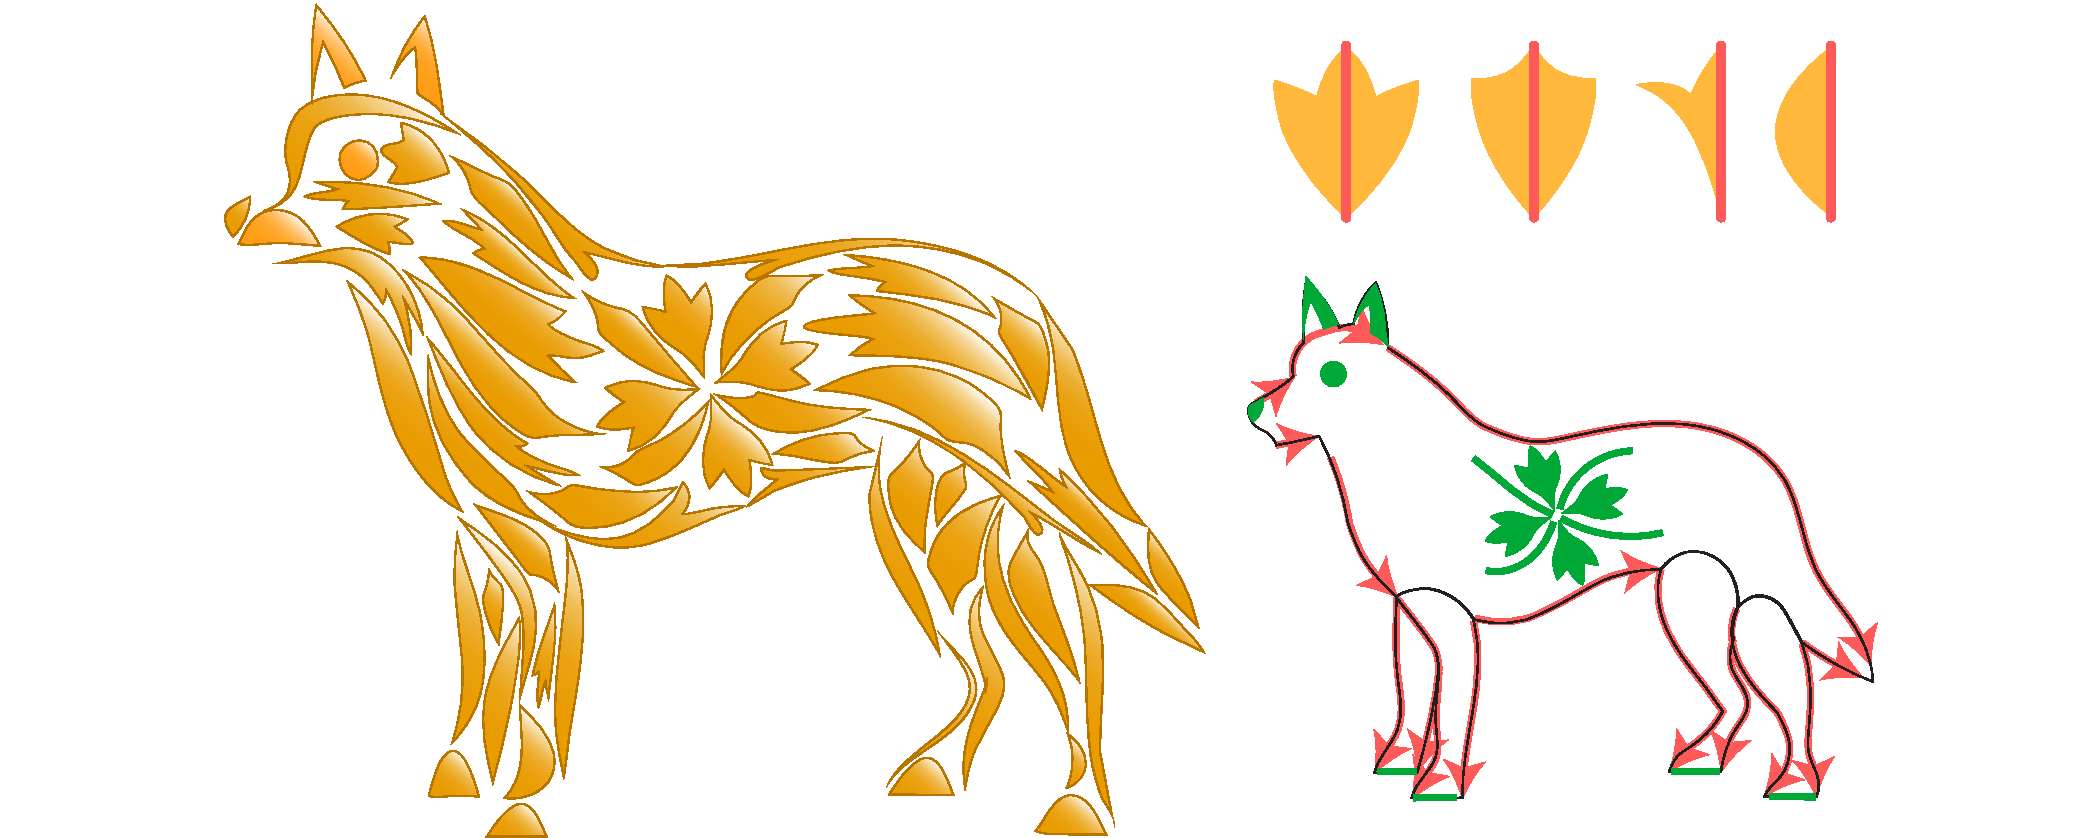
\includegraphics[width=6cm]{figures/flowpak/dog_flower.pdf}
\caption[A packing of a dog]
{A packing of a dog. The fixed elements, shown as green
	shapes in the diagram, are copied as-is to the output; fixed spines,
	shown as green paths, force the placement of new elements at the given
	locations.}
\label{result_dog}
\end{figure}

%FFFFFFFFFFFFFFF
\begin{figure} %BEAR OFFSET
\centering
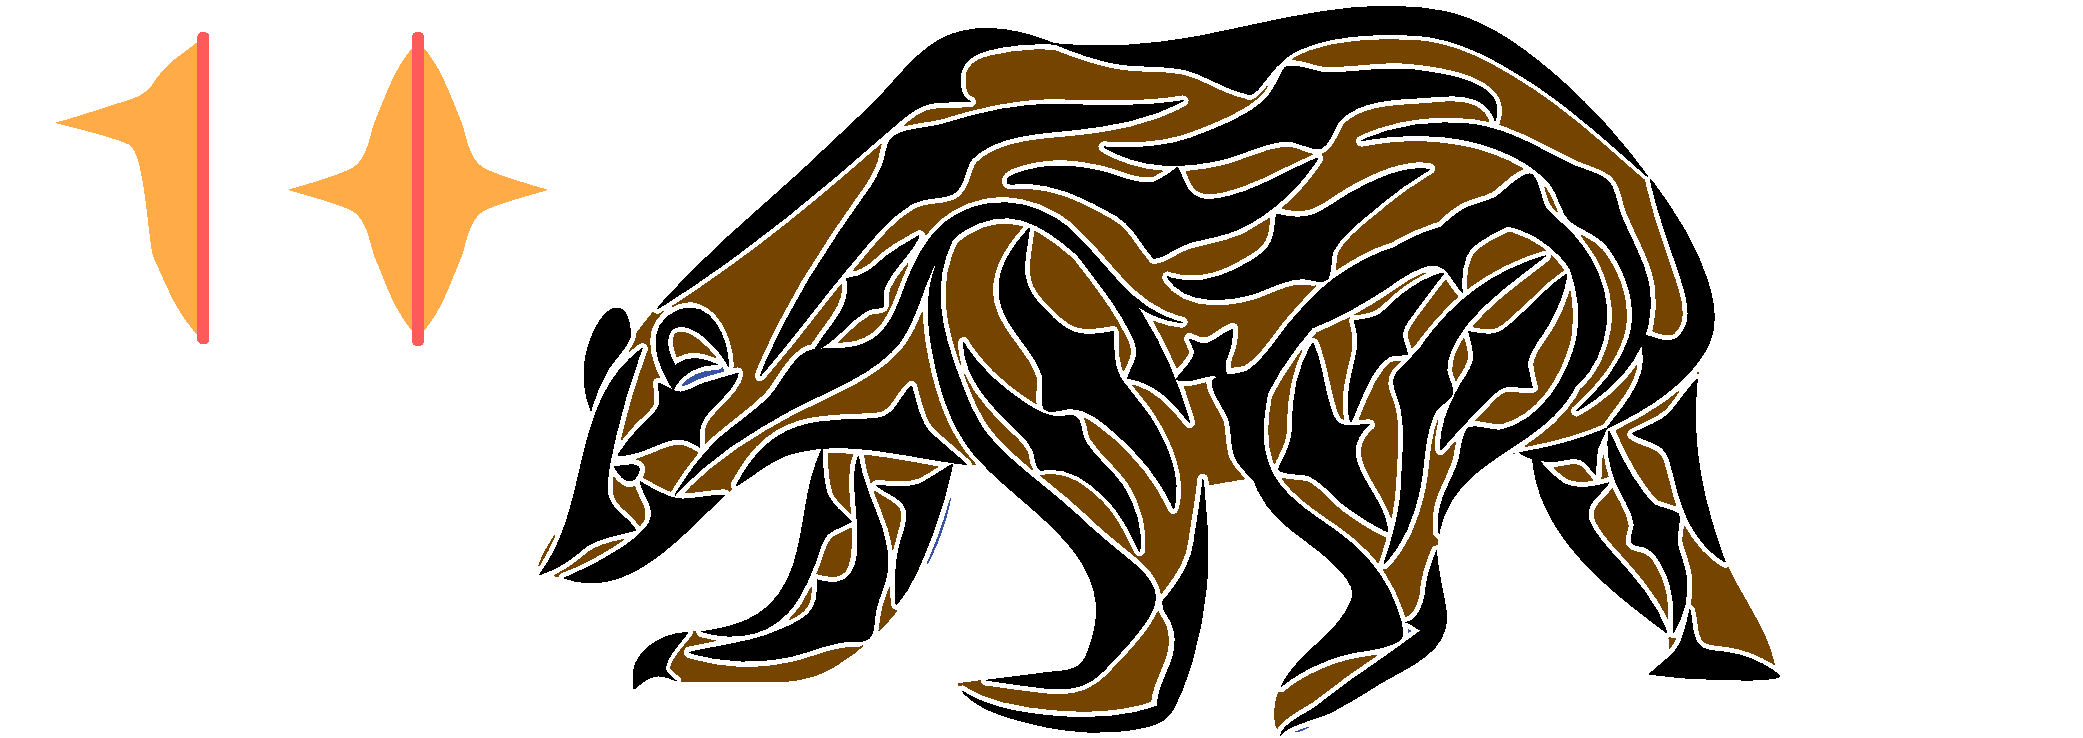
\includegraphics[width=6cm]{figures/flowpak/bear_offset_space.pdf}
\caption[A packing of a bear with elements created from negative space]
{A packing of the same container as in Figure~\ref{result_bear_leaves}.
	We place longer and sparser elements and synthesize additional forms to
	fill negative space.}
\label{result_bear_offset}
\end{figure}

%FFFFFFFFFFFFFFF
\begin{figure} %BIRD SQUARE
\centering
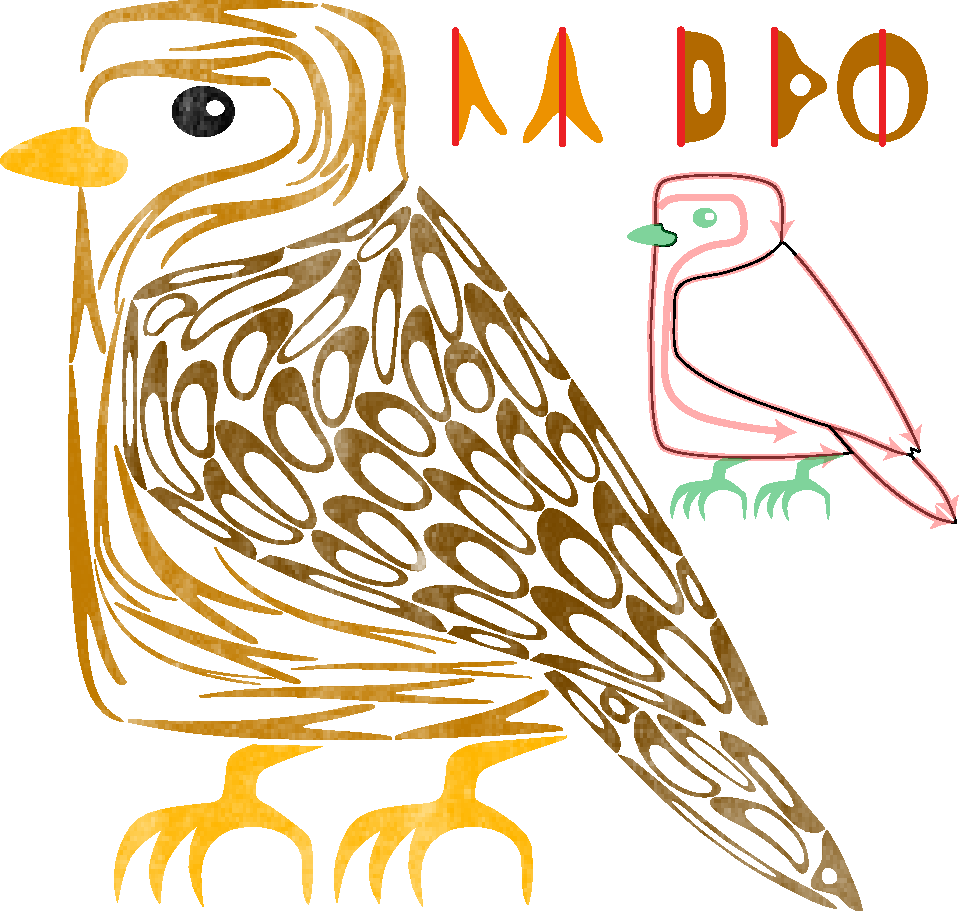
\includegraphics[width=6cm]{figures/flowpak/bird_square.pdf}
\caption[A packing of a bird]
{A packing of a bird, based on input provided by
	an artist.}
\label{bird_square}
\end{figure}

%%%%%%%%%%%%%%%%%%%%%%%%%%%%%%%%%%%%%%%%%%%%%%%%%%%%%%%%%%
%%%%%%%%%%%%%%%%%%%%%%%%%%%%%%%%%%%%%%%%%%%%%%%%%%%%%%%%%%
\section{Conclusions}
\label{flowpak_conclusions}
%%%%%%%%%%%%%%%%%%%%%%%%%%%%%%%%%%%%%%%%%%%%%%%%%%%%%%%%%%
%%%%%%%%%%%%%%%%%%%%%%%%%%%%%%%%%%%%%%%%%%%%%%%%%%%%%%%%%%
